\begin{figure}[H]
\centering
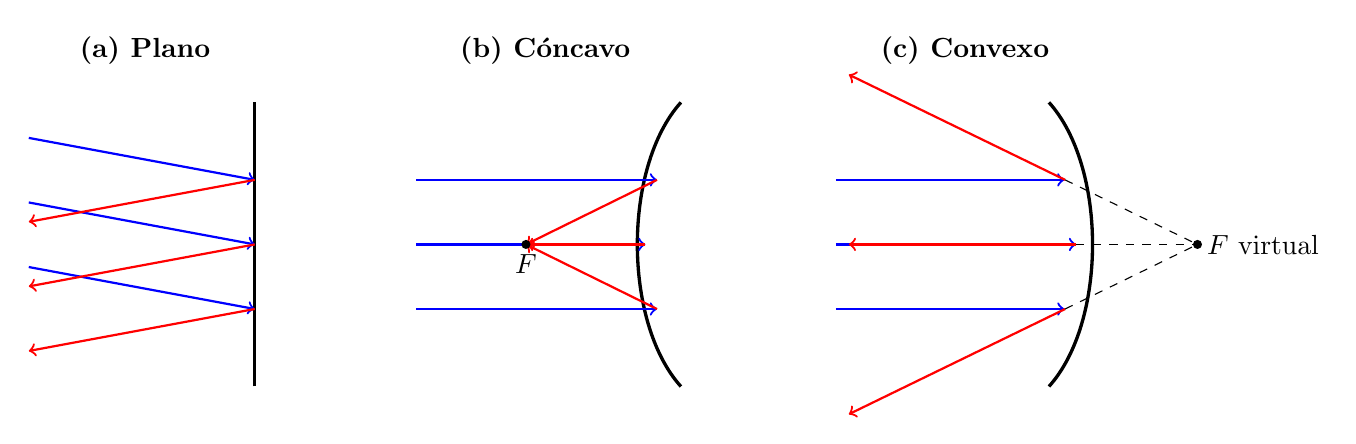
\begin{tikzpicture}[scale=0.82]
  \node[font=\bfseries] at (1.8,3) {(a) Plano};
  \draw[very thick] (3.5,-2.2) -- (3.5,2.2);
  \foreach \y in {-1,0,1}{
    \draw[->,blue,thick] (0,\y+0.65) -- (3.5,\y);
    \draw[->,red,thick] (3.5,\y) -- (0,\y-0.65);
  }
  \begin{scope}[xshift=6cm]
    \node[font=\bfseries] at (2,3) {(b) Cóncavo};
    \draw[very thick] (4.1,-2.2) .. controls (3.2,-1.2) and (3.2,1.2) .. (4.1,2.2);
    \foreach \y in {-1,0,1}{
      \draw[->,blue,thick] (0,\y) -- ({3.55+0.18*abs(\y)},\y);
      \draw[->,red,thick] ({3.55+0.18*abs(\y)},\y) -- (1.7,0);
    }
    \fill (1.7,0) circle (2pt) node[below] {$F$};
  \end{scope}
  \begin{scope}[xshift=12.5cm]
    \node[font=\bfseries] at (2,3) {(c) Convexo};
    \draw[very thick] (3.3,-2.2) .. controls (4.2,-1.2) and (4.2,1.2) .. (3.3,2.2);
    \foreach \y in {-1,0,1}{
      \draw[->,blue,thick] (0,\y) -- ({3.72-0.18*abs(\y)},\y);
    }
    \draw[->,red,thick] (3.55,1) -- (0.2,2.63);
    \draw[->,red,thick] (3.72,0) -- (0.2,0);
    \draw[->,red,thick] (3.55,-1) -- (0.2,-2.63);
    \draw[dashed] (3.55,1) -- (5.6,0);
    \draw[dashed] (3.72,0) -- (5.6,0);
    \draw[dashed] (3.55,-1) -- (5.6,0);
    \fill (5.6,0) circle (2pt) node[right] {$F$ virtual};
  \end{scope}
\end{tikzpicture}
\caption{Espejo plano, cóncavo convergente y convexo divergente.}
\end{figure}